\documentclass[12pt]{article}
\usepackage{graphicx}
\usepackage{booktabs}

\begin{document}


%%%%%%%%%%%%%%%%%%%%%%%%%%%%%%%%%%%%%%%%%%%%%%%%%%%%%%%%%%%%%%%%%%%%%%%%%%%%%%%

In this section, we present solutions for the model with heterogeneous harm under a subjective choice of dose-response function, at different levels of dose supply constraints. Our calibration is based on the initial efficacy results of the first effective COVID-19 vaccines and mass vaccination campaigns in late 2020 and throughout 2021, when all countries faced shortage of vaccines. We are interested in comparing three possible approaches to vaccination: giving full doses only, giving optimal partial doses, and varying the optimal dose as a function of harm.

Previously, in \cite{wiecek2021}, we demonstrated that fractional dosing with a fixed dose (that is, same lower dose used for all) can have large benefits under a range of realistic scenarios stylised after early COVID epidemics. Here, we expand on that work in two major ways. First, we want to characterise the solutions for harm-specific optimal dose: when risk is heterogeneous, how heterogeneous is the dose? Second, we investigate magnitude of marginal benefits of moving beyond fixed optimal dose to an age-specific one. We also extend the implications beyond single epidemic peak to long-run dynamics, where over time individuals lose immunity and are re-vaccinated.


\section{Calibration model}

To solve for optimal dose under variety of scenarios, we use a slightly modified version of the model we previously presented in \cite{wiecek_2021}. Here we just give a short exposition. 

We account for the dynamics of infection, mortality, and vaccination through a SEIRD-type compartmental epidemiological model, which is the workhorse of mathematical epidemiology.\footnote{We solve the model numerically using the \textit{odin} package in R \cite{odin}. While some simple compartmental models admit closed-form solutions, most realistic models, including ours, are too complex to solve analytically due to multiple compartments, age structure, and time-varying parameters. Therefore, we rely on numerical simulation to study the model's behavior and evaluate objective function for the dose optimisation problem.} 

The model divides the population into several compartments: susceptible ($S$), exposed ($E$), infectious ($I$), recovered ($R$), dead ($D$), vaccinated and protected ($P$), and vaccinated but not protected ($N$). Individuals move between these compartments based on a set of differential equations. The population is further stratified into age cohorts, as we will detail below.

The basic epidemic model is as follows. The rate at which susceptible individuals ($S + N$) become infected depends on their contact rates with infectious individuals, which are governed by a fixed contact matrix that specifies the frequency of interactions between different age groups. Once infected, individuals move from the exposed to the infectious compartment at a rate determined by the incubation period of the virus. They then either recover or die, with the proportion of deaths determined by age-specific infection fatality rates (IFRs). 

The basic reproductive number, $\mathcal{R}_0$, represents the average number of new infections generated by a single infected individual in a fully susceptible population. We consider two scenarios: a fast-growing outbreak ($\mathcal{R}_0 = 2$; in absence of vaccine infections peaking at about four months, about 55\% of population infected) and a slower-growing case ($\mathcal{R}_0 = 1.1$, infections slowly rise over 6 months, about 15\% of population infected). For an epidemic with $\mathcal{R}_0 = 1.1$ it's relatively easy to stop exponential growth by making about one in ten individuals immune.

Outputs for a few compartments of the model with $\mathcal{R}_0 = 2$, at different vaccination speeds (more on which below) are shown in Figure \ref{fig:example_model}. The model parameters(contact rates, incubation and infectious periods, pre-existing immunity, IFRs etc.) are based on empirical evidence for COVID-19, but, given the large heterogeneity in all parameters across countries, the example should be thought of as mainly illustrative. 

The initial cases we present assume no loss of immunity with time, which is appropriate for modeling a single epidemic outbreak. We revisit this assumption later in this section.



\subsection{Vaccine supply and vaccination model}

We consider vaccination of seven age groups: 20-29, 30-39, 40-49, 50-59, 60-69, 70-79, and 80+. We assume that under-20s do not get vaccinated since vaccines were initially approved for adults only. We assume vaccine hesitancy of 20\% in each age group, i.e. 80\% of people are willing to get vaccinated.\footnote{Overall, 80\% was the upper limit of vaccination coverage during COVID, but note that we use the same coverage in all age groups. In 2021 it was typical to reach over 80\% in highest risk groups and much lower in general population, but this pattern differed considerably across countries.}

We contrast two vaccination problems: ``dynamic'', where vaccinations occur during the epidemic, and ``static'', where vaccinations occur before the epidemic. The dynamic case is intended as a more realistic one in the case of COVID, but we also include the static case for contrast and because it's more flexible. In both cases we use the same SEIRD model.

In dynamic cases, the number of vaccinations is constant every day (e.g. 1\% of adult population vaccinated every day), to reflect supply and logistical constraints. Vaccination is reflected by moving individuals from the susceptible and recovered compartments to the $P$ compartment: each day we vaccinate a set proportion of total population $\delta$; a fraction $\phi(x)$ (efficacy) moves to protected compartment $P$ and remaining $1-\phi(x)$ move to compartment $N$.

While the details varied from country to country, to our knowledge all country-wide vaccination campaigns prioritised higher risk individuals. Therefore, to keep this example realistic, for dynamic cases we use a strict prioritisation strategy: 10-year age bands are vaccinated in descending order, each of them up to a point when there are no more willing individuals. 

In static cases, we consider several strategies for selecting age-group-specific dosage. This scheme is more flexible than in the dynamic cases: since we do not have to consider the order in which groups are vaccinated, prioritisation is meaningless. What matters is how the finite supply is divided among individuals.

This is done by changing the starting condition of the ODE system so that appropriate fraction of individuals are placed in $P$ and $N$ compartments. We discuss the potential loss of (natural and vaccine-induced) immunity later, but ignore it in the initial examples.

To keep these cases illustrative, we vary the quantity of vaccine available every day (dynamic cases) or total supply (static cases) through a wide range of values. This covers the heterogeneity in country-level supplies which occured during the COVID pandemic. For example, Israel was able to vaccinate a large fraction of its population in a manner of weeks, while most countries were only able to secure a very small supply of vaccine, which was then reserved for priority groups. In many cases these supply constraints were not alleviated until 2022. However, we also include the more extreme examples for illustrative purposes. To give some more precise examples for COVID:

\begin{itemize}

\item Wealthy countries that were at the front of the queue initially (circa January 2021) had enough doses to vaccinate a few percent of their population
\item As vaccination campaigns took off, these countries were vaccinating between 0.5\% and 1\% of their population. The UK and US fully vaccinated half of the population in the first half of 2021. Many EU countries started slowly and took several more months to reach that milestone. Typically the coverage of 60\%-80\% (depending on hesitancy) was reached within one year.
\item In poorer countries that had to rely on COVAX and donations, there was initially no supply; once vaccines were available, the vaccination rates were very slow. India (with large domestic supply) took 13 months to reach 50\% fully vaccinated, but Nigeria vaccinated 2\% in 2021 and then 25\% in 2022. 

\end{itemize}



\begin{figure}
\centering
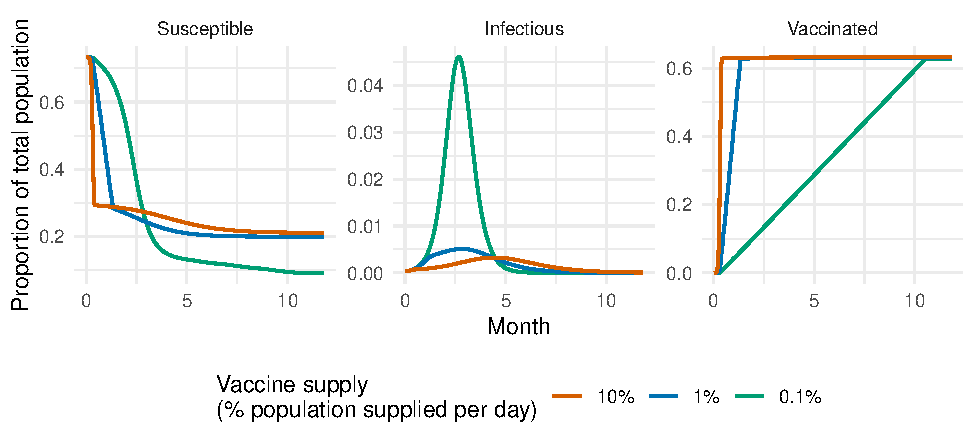
\includegraphics{figures/example_model.pdf}
\caption{Test}
\label{fig:example_model}
\end{figure}



\subsection{Dose-response function}

First, we assume that the net benefits function takes the form
$\phi(x) = Ax^\beta + Bx$ for $x \in [0,\infty)$. Our choice of $\phi(x)$ is twice differentiable and concave. We chose a subjective dose-response function as follows: first, assume that vaccine developers set full doses, $x^m=1$, to maximize expected net benefits such that $\phi'(1)=0$. At a full dose, we assumed the vaccine course would yield 95\% of maximum net benefits, $\phi(1)=0.95$, which is roughly level of efficacy that has been estimated for Moderna and Pfizer vaccines in December 2020; both vaccines have also reported no serious adverse events.

Second, at a half dose, $x=0.5$, we assumed some loss of efficacy, down to 80\% of maximum net benefits, $\phi(0.5)=0.8$. We then assumed that minimal acceptable level of efficacy (according to WHO's target product profile for COVID-19 vaccines) occurs at one-fifth of the dose and set $\phi(0.2) = 0.5$. At $x=0$, we expected the vaccine to yield no net benefits, $\phi(0)=0$.  Together these imply parameters $A=-25.3$, $\beta = 1.04$, and $B=26.3$. 

Our subjective choice of dose-response for this example is motivated by trial data and analysis we conducted in \cite{wiecek_pnas_2021}. Our analysis in that paper suggested that the subjective choice of dose-response curve for this example can be thought of as conservative with regards to loss of efficacy, but it's important to remember that this ignores viral variants.



\subsection{Heterogeneity in harm of infection and death}

We assume a discrete distribution of harm, which is driven by a combination of two risks; (1) a risk of infection: dynamic with time and age-specific (governed by the epidemiological model); (2) a risk death if infected (IFR): static, but also age-specific. Both IFR and infection risks vary in 10-year age bands. 


% REMOVE HIC VS LIC PERSPECTIVE? OR SAY "More on that below"

Older people have a much higher risk IFR than the younger adults.\footnote{While IFR varied from country to country and also changed over time, these simple estimates capture the main feature we are interested in illustrating here, that is, the degree of differences in risk across age groups.} The patterns also look different in low-income countries compared to high-income countries: in the former the mortality as a function of age was shown to be flatter than in the latter; the population pyramid is also a different shape. We include both LIC and HIC examples to illustrate how sensitive the model is to these differences.

A demonstration of an evolution of a single dynamic model is given in Figure 1. This is done under a fast-growing epidemic ($R_0 = 2$). We can clearly see that in this case a vaccination can have a decisive impact if enough people acquire vaccine-induced protection early enough in the outbreak.


\section{Magnitude of benefits from optimising}

For the rest of this section, we use non-linear optimisation solver to find optimal doses under a variety of scenarios.\footnote{We solve the differntial equations numerically using the \textit{odin} package in R. While some simple compartmental models admit closed-form solutions, most realistic models, including ours, are too complex to solve analytically, due to multiple compartments, age structure, and time-varying parameters. Therefore, we rely on numerical simulation to study the model's behavior and make quantitative predictions.} In the base case we vary three main variables:

%LICs, yes or no?

\begin{itemize}
\item daily vaccination speed (if vaccinating during epidemic) or total vaccine quantity (if vaccinating before),
\item slow-growing epidemic ($\mathcal{R}_0 = 1.1$) and fast-growing epidemic ($\mathcal{R}_0 = 2$),
\item heterogeneity in harm: using IFR typical of a high or a low income country
\end{itemize}

We can summarise the base case results in two ways: the magnitude of reductions and distribution with age. Figure \ref{fig:obj_f_solutions} focuses on magnitude, i.e. how the objective function (mortality) changes as if we optimise doses. This is crucial, because it directly addresses the central question of whether dose-stretching has potential save lives. We contrast four increasingly complex strategies of dosing:

% REMOVE THE INTERMEDIATE APPROACH (ON OR OFF) AND ADD COMMENTARY ON IT AS A FOOTNOTE

\begin{itemize}

\item using full doses (e.g., if supply is 10\% that means the top 10\% of the population with highest risk are vaccinated),
\item age-invariant fractional doses: we find the optimal fractional dose and vaccinate everyone with it
\item ``on or off`` fractional doses: we set one fractional dose and for each age group we either do not vaccinate, or vaccinate them with that fractional dose
\item age-specific optimal dose: we find a vector of optimal doses that varies across age groups

\end{itemize}

We include the invariant and ``on or off`` approaches to contrast simpler approaches to lower doses with more granular ones. When lowering doses in dynamic cases, we assume that daily number of vaccinees rises in inverse proportion to dose: e.g. if using 0.5 dose for all, we can vaccinate twice as many people every day. In other words, we do not consider any logistical constraints.

Figure \ref{fig:obj_f_solutions} contrasts fast-growth and slow-growth epidemics (left and right panels), as well as showing proportion of deaths reduced relative to no vaccination (top) and further improvements relative to the full dose strategy (bottom). Some of the values are given in Table \ref{table:obj_f}. 

Predictably, we find that vaccination with an effective vaccine can avert a large proportion of deaths (Figure \ref{fig:obj_f_solutions}, upper panels, black line); because the full doses are highly effective, at a certain level of coverage herd immunity is reached and there are nearly no deaths. Although that is not shown on the graph, which only uses relative quantities, for a slowly growing epidemic that point is achieved quickly: there is no exponential growth, and the burden quickly becomes negligible. 

Secondly, we also find that there are even larger benefits from fractionation in presence of supply constraints (if there are no constraints, we do not fractionate and the solutions converge to the same value). The relative improvements from more complicated strategies are U-shaped functions of supply (Figure \ref{fig:obj_f_solutions}, lower panels). This matches results presented in our earlier paper, but now with some further observations on age-specific optimal dosing. The further gains from it, compared to the ``uniform'' (age-invariant) fractional dosing are of course always larger (due to optimising over more parameters), but their magnitude depends on supply and type of epidemic. For example, with doses for only 5\% of population and in fast-growing epidemic, the deaths averted under age-optimal dosing are additional 10 percentage points higher than under age-invariant strategy (44\% compared to 34\%, see Table \ref{table:obj_f}) and 17 p.p. higher than under no fractionation (27\%). 

\begin{figure}
\label{fig:obj_f_solutions}
\centering
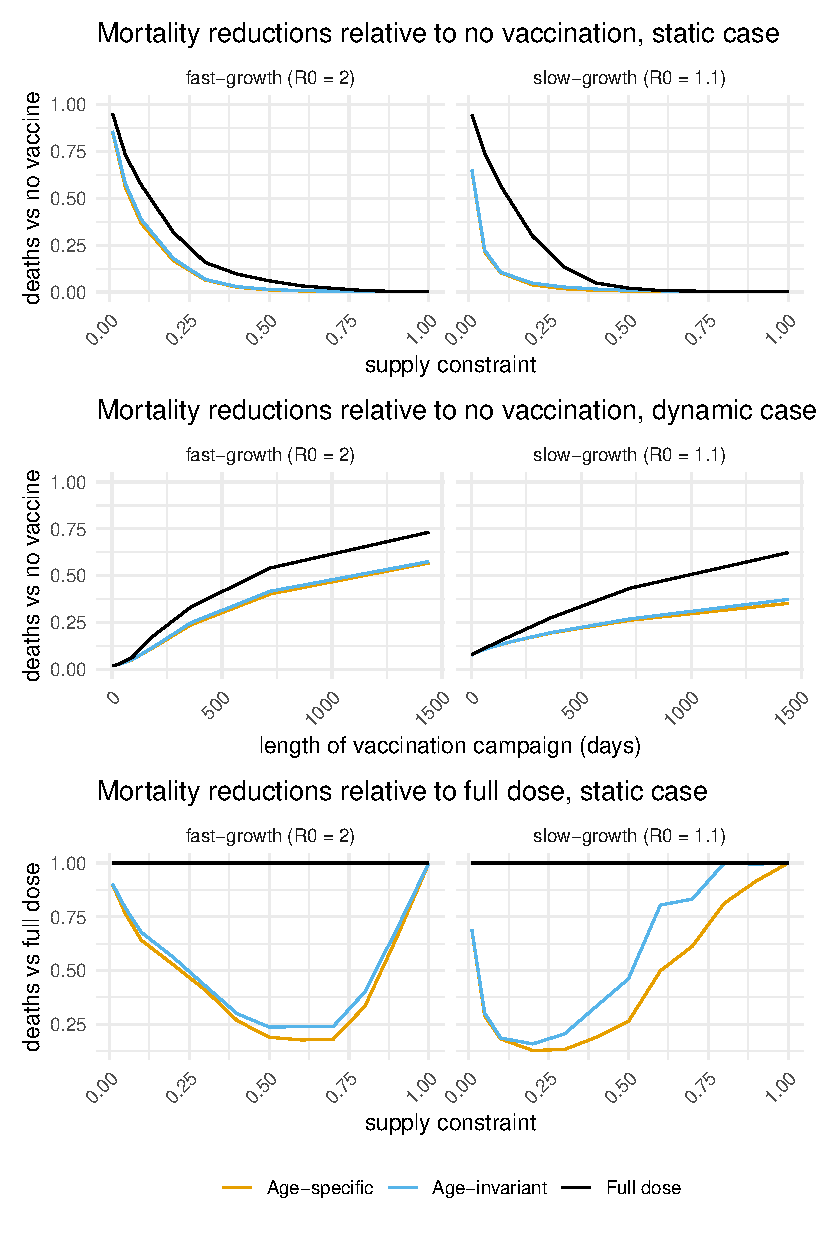
\includegraphics{figures/obj_f_solutions.pdf}
\caption{Magnitude of benefits from vaccination and switching to different lower dose strategies.}
\end{figure}

\begin{table}
\centering

\begin{tabular}{lrrrr}
\toprule
q & Age-optimal & Age-invariant & Binary choice & No f.d.\\
\midrule
\addlinespace[0.3em]
\multicolumn{5}{l}{\textbf{Fast-growing epidemic, R0 = 2}}\\
\hspace{1em}Supply = 0.05 & 0.56 & 0.66 & 0.58 & 0.73\\
\hspace{1em}Supply = 0.1 & 0.37 & 0.44 & 0.39 & 0.57\\
\hspace{1em}Supply = 0.2 & 0.17 & 0.18 & 0.18 & 0.32\\
\addlinespace[0.3em]
\multicolumn{5}{l}{\textbf{Slow-growing epidemic, R0 = 1.1}}\\
\hspace{1em}Supply = 0.05 & 0.21 & 0.23 & 0.22 & 0.74\\
\hspace{1em}Supply = 0.1 & 0.10 & 0.11 & 0.11 & 0.57\\
\hspace{1em}Supply = 0.2 & 0.04 & 0.05 & 0.05 & 0.30\\
\bottomrule
\end{tabular}

\caption{Underlying values for parts of Figure \ref{fig:age_solutions_both}.}
\label{table:obj_f}
\end{table}



\section{Optimal dose solutions}


%The slow-growth case can be thought of as one in which vaccination can prevent exponential growth. The fast-growing case is one where high coverage is needed to stop growth and where it may be best to focus on protecting high-risk individuals.

To see how the improvements are achieved and why they are only meaningful when supply is severly limited, we should look at the age-optimal solutions themselves. These are shown in Figure \ref{fig:age_solutions_both}.

When vaccinating before the epidemic (upper panels), the optimal strategy tends to distribute limited supply of vaccine to groups with high mortality risk and ignore the ``transmitting groups'', i.e. most solution vectors rise with age. That is because of steep differences in mortality risk and the fact that small quantities of vaccine are not able to slow the spread, even assuming sterilising immunity.\footnote{For slowly-growing epidemics with very small supply, we find an exception to this, where working-age adults are targetted for vaccination ahead of the elderly. That is because for it's easier to blunt the exponential growth when $\mathcal{R}_0$ is smaller. From the earlier figure we can see that a large majority of deaths can be averted by using lower doses.} When supply is very low, the optimal solution is proportional to IFR, which we plot on the top left panel in black dotted line.

For the dynamic problem (Figure \ref{fig:age_solutions_both}, lower panels), the optimal dose also rises with age when supply is constrained. (We do not show optimal dose in groups with less than 10\% coverage before the peak of the epidemic.) For particularly fast vaccination campaigns (3-6 months) it assumes an U shape; an intuitive explanation is that this is done to extend protection to youngest adults in order to slow down transmission. 

In general it seems the large differences in dosing in heterogeneous population (in both static and dynamic cases) occur in the case of severe supply constraints. When supply is really short, the optimal strategy is roughly proportional to mortality risk. When there is more supply, the optimal solutions tend to slope upwards with age, although often less steeply. However, in cases where the vaccine has impact on transmission (which we assumed here), there are no hard rules, because the protection against disease in those at highest risk of mortality has to be traded off against benefits of breaking transmission, which occurs in working age adults. Thus in realistic cases the vector of optimal dosing is not always monotonic with risk

% \begin{figure}
% \centering
% \includegraphics{figures/age_solutions_static.pdf}
% \caption{Test}
% \label{fig:age_solutions_static}
% \end{figure}
% 
% \begin{figure}
% \centering
% \includegraphics{figures/age_solutions_dynamic.pdf}
% \caption{Test}
% \label{fig:age_solutions_dynamic}
% \end{figure}

\begin{figure}
\centering
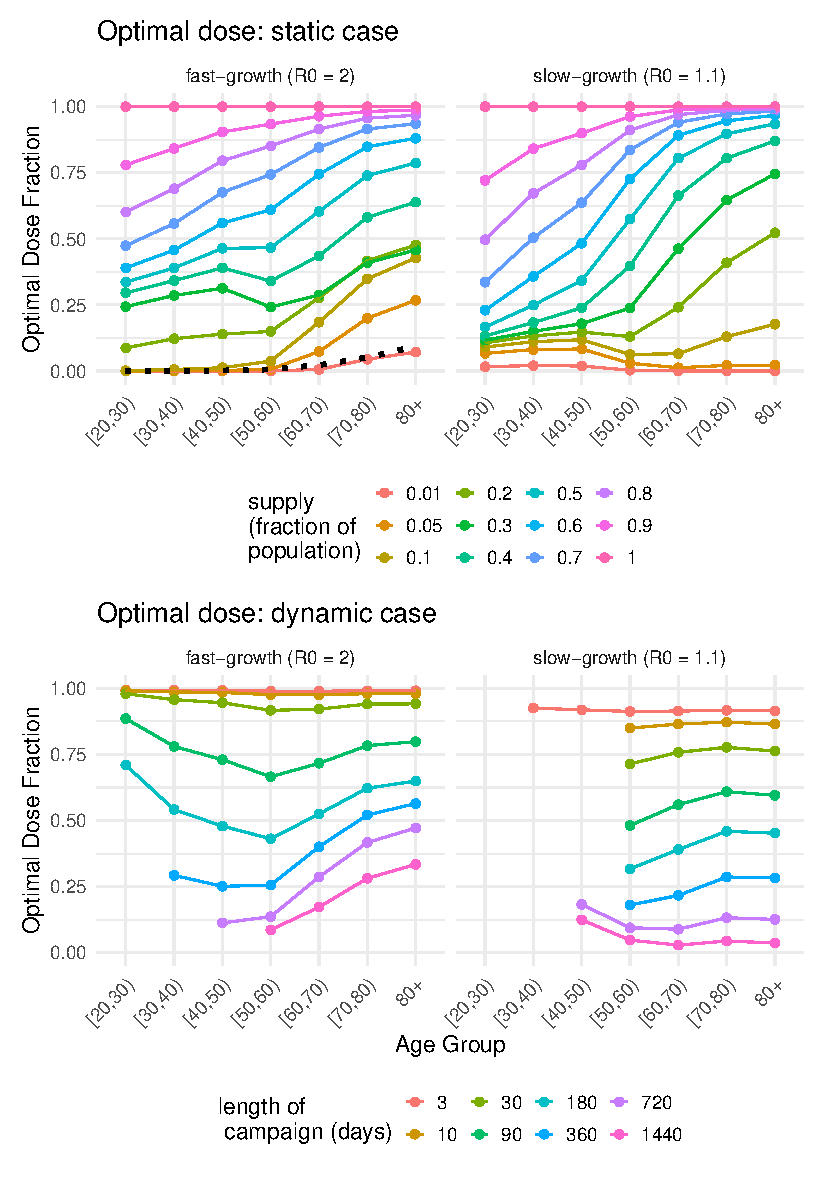
\includegraphics{figures/age_solutions_both.pdf}
\caption{Test}
\label{fig:age_solutions_both}
\end{figure}




\section{Additonal considerations}


\subsection{Different risk structure}

Figure \ref{fig:dose_sharing_nonepi} presents the results for low-income and high-income countries for comparison (see Appendix \ref{appx:supp} for the tables with exact numbers). We report results for a range of supply constraints $Q$ (proportion of the total population, excluding those under 20), which is the total units of vaccine divided by the population, and $p=0$. 

The result implies that it is optimal to give partial doses to all groups when the vaccine supply constraint binds ($Q<1$). Higher doses are given to those more at risk, because a small marginal gain in net benefits is more valuable (in averting harm) for the elderly than large gains in net benefits for the young. The optimal doses in HICs are lower than in LICs because the dispersion of harm is larger in HICs.


\section{What if risk is homogeneous?}


\section{A model with multiple vaccinations and re-infections}

So far we focused on a single epidemic outbreak, assuming no loss of immunity over time. However, for many infectious diseases, including COVID-19, immunity acquired through infection or vaccination will wane over time, leading to re-infections and the need for booster vaccinations. To capture these dynamics, we extend our model to simulate the epidemic over several years.

In this multi-season model, individuals in the recovered (R) and protected (P) compartments gradually lose their immunity and move back to the susceptible (S) compartment at a rate determined by the duration of immunity. This loss of immunity leads to a resurgence of infections in subsequent seasons, as the pool of susceptible individuals grows. To counter this, we introduce recurring vaccinations, where individuals are re-vaccinated at regular intervals to maintain a high level of population immunity.

% The inclusion of waning immunity and re-vaccination in the model has several important implications. First, it highlights the potential need for ongoing vaccination efforts to control the epidemic over a longer time horizon. Second, it allows us to examine the impact of different re-vaccination strategies, such as the timing and coverage of booster shots, on the long-term burden of the disease. Finally, it enables us to assess the robustness of optimal dose-stretching strategies in the face of changing epidemic dynamics and population immunity profiles.

% By simulating the epidemic over multiple seasons, we can gain insights into the long-term effectiveness of different vaccination strategies and inform policy decisions about the allocation of resources for ongoing disease control efforts. In the following sections, we will present the results of our multi-season simulations and discuss the implications for optimal dose-stretching policies in the context of waning immunity and re-infections.

It is important to consider this case separately, because the cases are likely to rebound in subsequent waves: for an endemic disease, preventing infections during a single outbreak means that the pool of susceptible individuals is going to be larger during the next period of exponential growth. In an extreme hypothetical case (and assuming no time discounting) this rebound can mean that benefits of a policy that optimises for reduced short-term infections are net zero. We showed elsewhere that this rebound effect has a sizeable impact in multi-year simulations of COVID epidemics (Więcek et al 2023).


\footnote{Beyond short-term efficacy and side effects, reducing the dose can also lead to shorter duration of protection. For this subjective example we assume that there is no significant impact on the duration of protection within the range of doses we consider. Moreover, as we mention below, some data suggest that our assumption on loss of efficacy may be conservative, but the lower net benefits at lower doses can also be interpreted as accounting not for loss of efficacy but shorter duration of immunity following a vaccination.}



\section{Summary of the case study}


% ADD STERILISING IMMUNITY PARAGRAPH

All of these numbers are intended to be illustrative. They use realistic ranges of parameters, but purposefully ignore some crucial features of COVID vaccines, such as development of variants, lower efficacy against transmission, behaviour change, and more. 

Indeed, our main point is to show that in situations where optimal dosing appears promising (i.e. we know \textit{a priori} that there are small loses from fractionation), the optimal vaccination strategy and magnitude of benefits still vary widely depending on epidemic and population factors. 

%However, we also show large benefits

For example, with doses for only 5\% of population and in fast-growing epidemic, the deaths averted under age-optimal dosing are additional 10 percentage points higher than under age-invariant strategy (44\% compared to 34\%, see Table \ref{table:obj_f}) and 17 p.p. higher than under no fractionation (27\%). 


\pagebreak


Moreover, some have suggested that lower doses, at least for some COVID-19 vaccines, may elicit more potent immunological response \cite{sanchez_limiting_2021}.



\end{document}
